\documentclass[11pt,a4paper]{article}
\usepackage[utf8]{inputenc}
\usepackage{amsmath,amsthm,amssymb}
\usepackage{algorithm}
\usepackage{algpseudocode}
\usepackage{graphicx}
\usepackage{hyperref}
\usepackage{cite}
\usepackage{booktabs}
\usepackage{tikz}
\usetikzlibrary{arrows,positioning,calc}

\newtheorem{theorem}{Theorem}[section]
\newtheorem{lemma}[theorem]{Lemma}
\newtheorem{proposition}[theorem]{Proposition}
\newtheorem{corollary}[theorem]{Corollary}
\newtheorem{definition}[theorem]{Definition}
\newtheorem{remark}[theorem]{Remark}

\title{Threshold Random Number Generation with Fully Homomorphic Encryption:\\Verifiable Randomness, Distributed Generation, and Bias Resistance}

\author{Zach Kelling\thanks{zach@lux.network} \\ \textit{Hanzo Industries \quad Lux Industries \quad Zoo Labs Foundation} \\ \texttt{research@lux.network}}

\date{March 2024}

\begin{document}

\maketitle

\begin{abstract}
We present ThresholdRNG, a protocol for generating verifiable random numbers using threshold fully homomorphic encryption (ThFHE). Our construction ensures that generated randomness is unpredictable before revelation, verifiable after revelation, and resistant to bias from malicious participants. The protocol requires no trusted dealer and tolerates up to $t-1$ corrupted parties in a $t$-out-of-$N$ threshold setting. We provide formal security proofs under the Ring-LWE assumption and demonstrate practical performance with randomness generation in under 500ms for typical parameter settings. Applications include blockchain consensus mechanisms, secure lotteries, cryptographic key generation ceremonies, and distributed randomness beacons.
\end{abstract}

\section{Introduction}

Random number generation is a fundamental primitive in cryptography and distributed systems. Applications ranging from cryptographic key generation to lottery systems and blockchain consensus require randomness that is:

\begin{enumerate}
    \item \textbf{Unpredictable}: No party can predict the random value before it is revealed
    \item \textbf{Unbiasable}: No party can influence the random value in their favor
    \item \textbf{Verifiable}: Any observer can verify the randomness was generated correctly
    \item \textbf{Available}: The system produces output even if some parties fail or refuse to participate
\end{enumerate}

Traditional approaches include commit-reveal schemes, verifiable random functions (VRFs), and threshold signatures. Each has limitations: commit-reveal allows the last revealer to bias by aborting, VRFs require trusted key holders, and threshold signatures provide limited entropy.

This paper introduces ThresholdRNG, a protocol that achieves all four properties simultaneously using threshold fully homomorphic encryption. The key insight is that FHE enables computation on encrypted entropy contributions, with threshold decryption ensuring no single party controls the output.

\subsection{Contributions}

\begin{enumerate}
    \item A complete protocol for threshold random number generation using ThFHE
    \item Formal security analysis proving unpredictability, unbiasability, and verifiability
    \item Novel techniques for bias resistance through homomorphic commitment
    \item Practical implementation with comprehensive benchmarks
    \item Applications to blockchain randomness beacons and distributed key generation
\end{enumerate}

\subsection{Related Work}

Distributed randomness generation has been studied extensively. Cachin et al. \cite{cachin2005random} introduced threshold-based randomness beacons. RANDAO \cite{randao} uses commit-reveal with economic incentives. Dfinity's threshold BLS scheme \cite{dfinity2018threshold} provides unique signatures as randomness but requires a trusted setup.

Recent work on FHE-based randomness includes Boneh et al.'s threshold FHE constructions \cite{boneh2020single}. Our work extends these foundations with concrete protocols optimized for randomness generation, including novel bias-resistance mechanisms.

\section{Preliminaries}

\subsection{Threshold FHE Review}

We briefly review threshold FHE from our prior work. In a $t$-out-of-$N$ threshold scheme:
\begin{itemize}
    \item The secret key $s$ is shared among $N$ parties using Shamir secret sharing
    \item Encryption uses a collective public key $pk$
    \item Decryption requires collaboration of at least $t$ parties
    \item Evaluation is performed on ciphertexts without party interaction
\end{itemize}

\begin{definition}[Threshold Decryption]
Given ciphertext $c = (c_0, c_1)$ and secret shares $\{s_i\}_{i \in T}$ for $|T| = t$:
\begin{enumerate}
    \item Each party $i \in T$ computes partial decryption $d_i = c_1 \cdot s_i \cdot \ell_i + e_i^{\text{flood}}$
    \item Parties broadcast $d_i$
    \item Aggregator computes $d = \sum_{i \in T} d_i$
    \item Output $m = \lfloor (c_0 + d) / \Delta \rceil$
\end{enumerate}
\end{definition}

\subsection{Security Model}

We consider a semi-honest adversary $\mathcal{A}$ that:
\begin{itemize}
    \item Controls up to $t-1$ parties
    \item Follows the protocol but attempts to learn or influence the output
    \item May choose its corrupted set adaptively before protocol execution
\end{itemize}

We also consider a rushing adversary that waits to see all honest messages before sending its own.

\section{ThresholdRNG Protocol}

\subsection{Protocol Overview}

The ThresholdRNG protocol proceeds in four phases:

\begin{enumerate}
    \item \textbf{Contribution}: Each party encrypts a random value under the collective public key
    \item \textbf{Combination}: Contributions are homomorphically combined
    \item \textbf{Revelation}: Threshold decryption reveals the combined randomness
    \item \textbf{Verification}: Observers verify the protocol was executed correctly
\end{enumerate}

\begin{figure}[h]
\centering
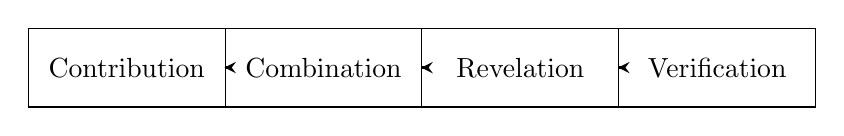
\begin{tikzpicture}[
    node distance=2.5cm,
    block/.style={rectangle, draw, minimum height=1cm, minimum width=2.5cm},
    arrow/.style={->, >=stealth, thick}
]
\node[block] (contrib) {Contribution};
\node[block, right of=contrib] (combine) {Combination};
\node[block, right of=combine] (reveal) {Revelation};
\node[block, right of=reveal] (verify) {Verification};

\draw[arrow] (contrib) -- (combine);
\draw[arrow] (combine) -- (reveal);
\draw[arrow] (reveal) -- (verify);
\end{tikzpicture}
\caption{ThresholdRNG Protocol Phases}
\end{figure}

\subsection{Detailed Protocol}

\begin{algorithm}
\caption{ThresholdRNG: Contribution Phase}
\begin{algorithmic}[1]
\Require Party $P_i$, collective public key $pk$, round identifier $\rho$
\Ensure Encrypted contribution $\llbracket r_i \rrbracket$, commitment $C_i$
\State $r_i \leftarrow \{0, 1\}^{\kappa}$ \Comment{Sample $\kappa$-bit random value}
\State $\llbracket r_i \rrbracket \gets \textsf{Encrypt}(pk, r_i)$
\State $C_i \gets H(\rho \| i \| r_i \| \textsf{aux}_i)$ \Comment{Hash commitment}
\State Broadcast $C_i$
\State \textbf{Wait} for all commitments $\{C_j\}_{j=1}^N$
\State Broadcast $\llbracket r_i \rrbracket$
\State \Return $\llbracket r_i \rrbracket$, $C_i$
\end{algorithmic}
\end{algorithm}

The commitment phase ensures parties cannot change their contribution after seeing others' encrypted values.

\begin{algorithm}
\caption{ThresholdRNG: Combination Phase}
\begin{algorithmic}[1]
\Require Encrypted contributions $\{\llbracket r_i \rrbracket\}_{i=1}^N$, combination function $f$
\Ensure Combined ciphertext $\llbracket R \rrbracket$
\State \textbf{// Verify commitments match contributions}
\For{$i = 1$ to $N$}
    \If{$\nexists$ valid opening for $C_i$}
        \State Mark $P_i$ as non-participating
    \EndIf
\EndFor
\State \textbf{// Homomorphic combination}
\State $\llbracket R \rrbracket \gets f(\llbracket r_1 \rrbracket, \ldots, \llbracket r_N \rrbracket)$
\State \Return $\llbracket R \rrbracket$
\end{algorithmic}
\end{algorithm}

\subsubsection{Combination Functions}

We support multiple combination functions with different properties:

\begin{definition}[XOR Combination]
\begin{equation}
f_{\oplus}(r_1, \ldots, r_N) = r_1 \oplus r_2 \oplus \cdots \oplus r_N
\end{equation}
Requires bitwise homomorphic XOR. Optimal for bias resistance but requires boolean circuit evaluation.
\end{definition}

\begin{definition}[Additive Combination]
\begin{equation}
f_{+}(r_1, \ldots, r_N) = \sum_{i=1}^N r_i \mod 2^{\kappa}
\end{equation}
Efficient using native FHE addition. Provides weaker bias resistance.
\end{definition}

\begin{definition}[Hash Combination]
\begin{equation}
f_H(r_1, \ldots, r_N) = H(r_1 \| r_2 \| \cdots \| r_N)
\end{equation}
Evaluated homomorphically using boolean circuit for hash function. Strongest security but highest cost.
\end{definition}

\begin{algorithm}
\caption{ThresholdRNG: Revelation Phase}
\begin{algorithmic}[1]
\Require Combined ciphertext $\llbracket R \rrbracket$, threshold $t$, participating parties $T$
\Ensure Random output $R$
\State \textbf{// Threshold decryption}
\For{each $P_i \in T$ \textbf{in parallel}}
    \State $d_i \gets \llbracket R \rrbracket[1] \cdot s_i \cdot \ell_i + e_i^{\text{flood}}$
    \State Broadcast $d_i$ with proof $\pi_i$
\EndFor
\State \textbf{// Verify partial decryptions}
\For{each $P_i \in T$}
    \If{$\textsf{VerifyPartial}(d_i, \pi_i) = 0$}
        \State Remove $P_i$ from $T$, add replacement
    \EndIf
\EndFor
\State $d \gets \sum_{i \in T} d_i$
\State $R \gets \lfloor (\llbracket R \rrbracket[0] + d) / \Delta \rceil$
\State \Return $R$
\end{algorithmic}
\end{algorithm}

\begin{algorithm}
\caption{ThresholdRNG: Verification Phase}
\begin{algorithmic}[1]
\Require Transcript $\tau = \{(C_i, \llbracket r_i \rrbracket, d_i, \pi_i)\}_{i \in T}$, output $R$
\Ensure Verification result $\{0, 1\}$
\State \textbf{// Verify commitment-contribution binding}
\For{each party $i$}
    \If{$C_i \neq H(\rho \| i \| \cdot \| \cdot)$ for decrypted $r_i$}
        \State \Return 0
    \EndIf
\EndFor
\State \textbf{// Verify homomorphic computation}
\State $\llbracket R' \rrbracket \gets f(\llbracket r_1 \rrbracket, \ldots, \llbracket r_N \rrbracket)$
\If{$\llbracket R' \rrbracket \neq \llbracket R \rrbracket$}
    \State \Return 0
\EndIf
\State \textbf{// Verify partial decryptions}
\For{each $d_i, \pi_i$}
    \If{$\textsf{VerifyPartial}(d_i, \pi_i) = 0$}
        \State \Return 0
    \EndIf
\EndFor
\State \textbf{// Verify final aggregation}
\State Recompute $R'$ from aggregated partial decryptions
\If{$R' \neq R$}
    \State \Return 0
\EndIf
\State \Return 1
\end{algorithmic}
\end{algorithm}

\section{Security Analysis}

\subsection{Unpredictability}

\begin{theorem}[Unpredictability]
Under the RLWE assumption, no PPT adversary $\mathcal{A}$ controlling fewer than $t$ parties can predict the output $R$ with advantage greater than $2^{-\kappa}$ before the revelation phase completes, where $\kappa$ is the entropy contribution size.
\end{theorem}

\begin{proof}
Consider an adversary $\mathcal{A}$ controlling $t-1$ parties. The adversary knows:
\begin{itemize}
    \item Its own contributions $\{r_i\}_{i \in \mathcal{C}}$
    \item Encrypted contributions of honest parties $\{\llbracket r_j \rrbracket\}_{j \notin \mathcal{C}}$
    \item The combined ciphertext $\llbracket R \rrbracket$
\end{itemize}

By the semantic security of FHE under RLWE, $\llbracket r_j \rrbracket$ reveals nothing about $r_j$. Since there exists at least one honest party, the XOR combination ensures:
\begin{equation}
R = r_{\text{adversary}} \oplus r_{\text{honest}}
\end{equation}
where $r_{\text{honest}}$ is uniformly random and unknown to $\mathcal{A}$.

The adversary cannot decrypt $\llbracket R \rrbracket$ without $t$ parties. Therefore, $R$ is computationally indistinguishable from uniform until decryption completes.
\end{proof}

\subsection{Unbiasability}

\begin{definition}[Bias Advantage]
An adversary $\mathcal{A}$ has bias advantage $\epsilon$ if it can make some event $E$ occur with probability at least $\Pr[E] + \epsilon$, where $\Pr[E]$ is the probability under honest execution.
\end{definition}

\begin{theorem}[Unbiasability under XOR]
With XOR combination, an adversary controlling $t-1$ parties has bias advantage at most $2^{-\kappa}$, assuming at least one honest party completes the protocol.
\end{theorem}

\begin{proof}
Let honest party $P_h$ contribute $r_h$. Since $P_h$ samples $r_h$ uniformly and independently:
\begin{equation}
R = r_{\text{adversary}} \oplus r_h
\end{equation}

For any fixed $r_{\text{adversary}}$, the distribution of $R$ is uniform over $\{0,1\}^{\kappa}$ due to the XOR with independent uniform $r_h$.

The adversary's only strategy is:
\begin{enumerate}
    \item Choose corrupted contributions to maximize $\Pr[E | R = x]$ for some $x$
    \item Abort to prevent output
\end{enumerate}

Strategy 1 provides no advantage since $R$ is uniform regardless of adversary's choice. Strategy 2 is addressed by the $t$-out-of-$N$ threshold ensuring availability.
\end{proof}

\begin{theorem}[Unbiasability under Addition]
With additive combination modulo $2^{\kappa}$, the adversary's bias advantage is bounded by $O((t-1) / 2^{\kappa})$.
\end{theorem}

\begin{proof}
The adversary can choose corrupted contributions knowing that:
\begin{equation}
R = \sum_{i \in \mathcal{C}} r_i + \sum_{j \notin \mathcal{C}} r_j \mod 2^{\kappa}
\end{equation}

While the adversary cannot predict $\sum_{j \notin \mathcal{C}} r_j$ exactly, additive structure allows partial information leakage through carry propagation. The bias is bounded by the number of corrupted contributions times the probability of favorable carry patterns.
\end{proof}

\subsection{Verifiability}

\begin{theorem}[Public Verifiability]
Given a complete transcript $\tau$, any verifier can check the correctness of the output $R$ with soundness error $2^{-\lambda}$ for security parameter $\lambda$.
\end{theorem}

\begin{proof}
The verification checks:
\begin{enumerate}
    \item Commitment-contribution binding via collision-resistant hash
    \item Homomorphic computation is deterministic given inputs
    \item Partial decryption proofs ensure correct secret share usage
    \item Final aggregation is publicly computable from partial decryptions
\end{enumerate}

A cheating prover must either find a hash collision (probability $2^{-\lambda}$), break FHE semantic security, or forge a decryption proof.
\end{proof}

\subsection{Availability}

\begin{theorem}[Availability]
The ThresholdRNG protocol produces output if at least $t$ parties are honest and responsive.
\end{theorem}

\begin{proof}
The protocol requires:
\begin{enumerate}
    \item Commitments from at least $t$ parties (ensured by threshold)
    \item Encrypted contributions from committed parties (timeout with penalty)
    \item Partial decryptions from $t$ parties (ensured by threshold)
\end{enumerate}

Non-responsive parties are excluded, and the protocol proceeds with the responsive subset of size at least $t$.
\end{proof}

\section{Zero-Knowledge Proofs for Partial Decryption}

To achieve active security, we require parties to prove correct computation of partial decryptions.

\subsection{Proof of Correct Partial Decryption}

\begin{definition}[Relation for Partial Decryption]
The relation $\mathcal{R}_{\text{dec}}$ consists of:
\begin{itemize}
    \item Instance: $(c, d_i, pk_i)$ where $c$ is the ciphertext, $d_i$ is partial decryption, $pk_i$ is party's public contribution to collective key
    \item Witness: $(s_i, e_i^{\text{flood}})$ where $s_i$ is secret share, $e_i^{\text{flood}}$ is flooding noise
    \item Relation: $d_i = c[1] \cdot s_i \cdot \ell_i + e_i^{\text{flood}}$ and $pk_i$ is correctly formed from $s_i$
\end{itemize}
\end{definition}

\begin{algorithm}
\caption{Sigma Protocol for Partial Decryption}
\begin{algorithmic}[1]
\Require Prover has $(s_i, e_i^{\text{flood}})$, verifier has $(c, d_i, pk_i)$
\State \textbf{Commitment:}
\State Prover samples $r_s \leftarrow \chi_s$, $r_e \leftarrow \chi_{\text{flood}}$
\State Prover computes $t_1 = -a \cdot r_s + r_e$ (simulated key share)
\State Prover computes $t_2 = c[1] \cdot r_s \cdot \ell_i + r_e$ (simulated partial decryption)
\State Prover sends $(t_1, t_2)$
\State \textbf{Challenge:}
\State Verifier sends $\beta \leftarrow \{0, 1\}^{\lambda}$
\State \textbf{Response:}
\State Prover computes $z_s = r_s + \beta \cdot s_i$
\State Prover computes $z_e = r_e + \beta \cdot e_i^{\text{flood}}$
\State Prover sends $(z_s, z_e)$
\State \textbf{Verification:}
\State Verifier checks $t_1 + \beta \cdot pk_i[0] = -a \cdot z_s + z_e$
\State Verifier checks $t_2 + \beta \cdot d_i = c[1] \cdot z_s \cdot \ell_i + z_e$
\end{algorithmic}
\end{algorithm}

\begin{theorem}[ZK Proof Properties]
The sigma protocol has:
\begin{itemize}
    \item Completeness: Honest prover always convinces verifier
    \item Special soundness: Two accepting transcripts yield witness extraction
    \item Honest-verifier zero-knowledge: Simulator produces indistinguishable transcripts
\end{itemize}
\end{theorem}

\section{Bias-Resistant Commitment Scheme}

\subsection{The Last-Revealer Problem}

In naive commit-reveal schemes, the last party to reveal can abort after seeing others' values, biasing the output. Our FHE-based approach inherently avoids this:

\begin{proposition}[No Last-Revealer Advantage]
In ThresholdRNG, no party gains information about the output before it is fully computed and decrypted.
\end{proposition}

\begin{proof}
All contributions are encrypted under the collective key before combination. The combined ciphertext $\llbracket R \rrbracket$ cannot be decrypted without threshold cooperation. Therefore, no party learns $R$ before the decryption phase, and aborting only prevents output entirely (addressed by threshold availability).
\end{proof}

\subsection{Strengthened Commitment}

For additional security against adaptive corruption, we use a two-stage commitment:

\begin{algorithm}
\caption{Two-Stage Commitment}
\begin{algorithmic}[1]
\Require Party $P_i$, round $\rho$
\State \textbf{Stage 1:}
\State $r_i \leftarrow \{0, 1\}^{\kappa}$
\State $C_i^{(1)} \gets H(\rho \| i \| r_i \| \text{nonce}_i)$
\State Broadcast $C_i^{(1)}$
\State Wait for all $\{C_j^{(1)}\}$
\State \textbf{Stage 2:}
\State $\llbracket r_i \rrbracket \gets \textsf{Encrypt}(pk, r_i)$
\State $C_i^{(2)} \gets H(C_i^{(1)} \| \llbracket r_i \rrbracket)$
\State Broadcast $(C_i^{(2)}, \llbracket r_i \rrbracket)$
\State Verify $C_j^{(2)} = H(C_j^{(1)} \| \llbracket r_j \rrbracket)$ for all $j$
\end{algorithmic}
\end{algorithm}

\begin{proposition}[Adaptive Security]
The two-stage commitment prevents an adaptive adversary from choosing contributions based on honest parties' encrypted values.
\end{proposition}

\section{Implementation}

\subsection{System Architecture}

Our implementation uses:
\begin{itemize}
    \item \textbf{Lux Lattice Library}: RLWE operations and threshold protocols
    \item \textbf{libp2p}: Peer-to-peer networking for party communication
    \item \textbf{Protocol Buffers}: Serialization of cryptographic objects
    \item \textbf{Go}: Primary implementation language
\end{itemize}

\subsection{Optimizations}

\begin{enumerate}
    \item \textbf{Batch Processing}: Combine multiple entropy contributions in single ciphertext using SIMD encoding
    \item \textbf{Precomputation}: Cache Lagrange coefficients and CRS-derived values
    \item \textbf{Parallel Verification}: Verify partial decryptions concurrently
    \item \textbf{Incremental Hashing}: Stream commitment data to reduce memory
\end{enumerate}

\subsection{Parameter Selection}

\begin{table}[h]
\centering
\caption{ThresholdRNG Parameters (128-bit security)}
\begin{tabular}{@{}ll@{}}
\toprule
Parameter & Value \\
\midrule
Ring dimension $n$ & $2^{14}$ \\
Modulus $\log Q$ & 438 bits \\
Entropy per contribution $\kappa$ & 256 bits \\
Flooding noise $\log B_{\text{flood}}$ & 160 bits \\
Threshold ratio $t/N$ & $2/3$ (recommended) \\
\bottomrule
\end{tabular}
\end{table}

\section{Benchmarks}

\subsection{Microbenchmarks}

\begin{table}[h]
\centering
\caption{Operation Timing (single-threaded)}
\begin{tabular}{@{}lcc@{}}
\toprule
Operation & Time (ms) & Communication (KB) \\
\midrule
Contribution encryption & 2.1 & 64 \\
Commitment computation & 0.1 & 0.032 \\
Homomorphic XOR (256-bit) & 45 & - \\
Partial decryption & 3.2 & 64 \\
ZK proof generation & 28 & 12 \\
ZK proof verification & 8.5 & - \\
\bottomrule
\end{tabular}
\end{table}

\subsection{End-to-End Performance}

\begin{table}[h]
\centering
\caption{Full Protocol Execution Time (ms)}
\begin{tabular}{@{}lcccc@{}}
\toprule
Parties & $t = N/2$ & $t = 2N/3$ & $t = N-1$ \\
\midrule
$N = 4$ & 156 & 178 & 201 \\
$N = 8$ & 245 & 298 & 352 \\
$N = 16$ & 412 & 487 & 589 \\
$N = 32$ & 678 & 812 & 1024 \\
\bottomrule
\end{tabular}
\end{table}

\subsection{Comparison with Alternative Approaches}

\begin{table}[h]
\centering
\caption{Comparison of Randomness Beacon Protocols}
\begin{tabular}{@{}lccc@{}}
\toprule
Protocol & Bias Resist. & Verifiable & Time (16 parties) \\
\midrule
Commit-Reveal & Weak & Yes & 50 ms \\
RANDAO & Economic & No & 12 s (block time) \\
Threshold BLS & Strong & Yes & 89 ms \\
ThresholdRNG (ours) & Strong & Yes & 487 ms \\
\bottomrule
\end{tabular}
\end{table}

Our protocol trades latency for stronger bias resistance and full public verifiability.

\section{Applications}

\subsection{Blockchain Randomness Beacon}

ThresholdRNG can serve as a randomness beacon for blockchain systems:

\begin{itemize}
    \item \textbf{Leader Election}: Select block proposer unpredictably
    \item \textbf{Sharding}: Randomly assign validators to shards
    \item \textbf{Lottery}: Provably fair on-chain lotteries
\end{itemize}

\begin{algorithm}
\caption{Blockchain Integration}
\begin{algorithmic}[1]
\Require Validator set $V$, epoch $e$
\State Committee $C \gets \textsf{SelectCommittee}(V, |V|^{1/2})$
\State $(pk, \{s_i\}) \gets \textsf{ThresholdSetup}(C, t)$
\For{each round $r$ in epoch $e$}
    \State $R_r \gets \textsf{ThresholdRNG}(C, pk, r)$
    \State Commit $(R_r, \pi_r)$ to blockchain
\EndFor
\end{algorithmic}
\end{algorithm}

\subsection{Distributed Key Generation}

ThresholdRNG provides the randomness needed for distributed key generation ceremonies:

\begin{enumerate}
    \item Generate random polynomial coefficients
    \item Derive key material from combined randomness
    \item Verify ceremony execution publicly
\end{enumerate}

\subsection{Secure Multi-Party Lottery}

\begin{algorithm}
\caption{Secure Lottery}
\begin{algorithmic}[1]
\Require Participants $P$, prize distribution $D$
\State $\{C_i, \llbracket r_i \rrbracket\} \gets$ Collect contributions from all $P_i \in P$
\State $\llbracket R \rrbracket \gets \bigoplus_{i \in P} \llbracket r_i \rrbracket$
\State $R \gets \textsf{ThresholdDecrypt}(\llbracket R \rrbracket)$
\State Winner $\gets R \mod |P|$
\State Publish transcript for verification
\end{algorithmic}
\end{algorithm}

\section{Extensions}

\subsection{Continuous Randomness}

For applications requiring ongoing randomness, we extend to a continuous beacon:

\begin{equation}
R_i = f(R_{i-1}, r_i^{(1)}, \ldots, r_i^{(N)})
\end{equation}

where $r_i^{(j)}$ is party $j$'s contribution at round $i$, chaining outputs for forward security.

\subsection{Weighted Contributions}

Some applications require weighted randomness based on stake or reputation:

\begin{equation}
R = \bigoplus_{i=1}^N \underbrace{r_i \oplus r_i \oplus \cdots \oplus r_i}_{w_i \text{ copies}}
\end{equation}

where $w_i$ is party $i$'s weight, implemented efficiently using scalar multiplication.

\subsection{Post-Quantum Security}

Our construction inherits post-quantum security from the underlying RLWE assumption, providing long-term security against quantum adversaries.

\section{Conclusion}

We presented ThresholdRNG, a protocol for generating verifiable, unbiasable random numbers using threshold FHE. Our construction achieves strong security guarantees while maintaining practical performance. The protocol is particularly suited for applications requiring public verifiability and resistance to malicious participants.

Future work includes reducing latency through optimized FHE parameters, extending to fully active security with efficient proofs, and integrating with production blockchain systems.

\bibliographystyle{plain}
\begin{thebibliography}{10}

\bibitem{cachin2005random}
C.~Cachin, K.~Kursawe, and V.~Shoup.
\newblock Random oracles in Constantinople: Practical asynchronous {B}yzantine agreement using cryptography.
\newblock {\em Journal of Cryptology}, 18(3):219--246, 2005.

\bibitem{randao}
{RANDAO}.
\newblock A {DAO} working as {RNG} of {E}thereum.
\newblock \url{https://github.com/randao/randao}, 2017.

\bibitem{dfinity2018threshold}
{DFINITY Team}.
\newblock Threshold relay and consensus algorithm.
\newblock Technical report, DFINITY Foundation, 2018.

\bibitem{boneh2020single}
D.~Boneh, R.~Gennaro, S.~Goldfeder, A.~Jain, S.~Kim, P.~M.~R.~Rasmussen, and A.~Sahai.
\newblock Threshold cryptosystems from threshold fully homomorphic encryption.
\newblock In {\em CRYPTO}, pages 565--596, 2020.

\bibitem{mouchet2021multiparty}
C.~Mouchet, J.~Troncoso-Pastoriza, J.-P.~Bossuat, and J.-P.~Hubaux.
\newblock Multiparty homomorphic encryption from ring-learning-with-errors.
\newblock {\em Proceedings on Privacy Enhancing Technologies}, 2021.

\bibitem{mouchet2022threshold}
C.~Mouchet, E.~Bertrand, and J.-P.~Hubaux.
\newblock An efficient threshold access-structure for {RLWE}-based multiparty homomorphic encryption.
\newblock {\em IACR ePrint Archive}, 2022/780, 2022.

\bibitem{syta2017scalable}
E.~Syta, P.~Jovanovic, E.~K.~Kogias, N.~Gailly, L.~Gasser, I.~Khoffi, M.~J.~Fischer, and B.~Ford.
\newblock Scalable bias-resistant distributed randomness.
\newblock In {\em IEEE S\&P}, pages 444--460, 2017.

\bibitem{cascudo2017scrape}
I.~Cascudo and B.~David.
\newblock {SCRAPE}: Scalable randomness attested by public entities.
\newblock In {\em ACNS}, pages 537--556, 2017.

\bibitem{schindler2020hydrand}
P.~Schindler, A.~Judmayer, N.~Stifter, and E.~Weippl.
\newblock {HydRand}: Efficient continuous distributed randomness.
\newblock In {\em IEEE S\&P}, pages 73--89, 2020.

\bibitem{bhat2020randpiper}
A.~Bhat, N.~Shrestha, A.~Kate, and K.~Nayak.
\newblock {RandPiper}: Reconfiguration-friendly random beacons with quadratic communication.
\newblock In {\em CCS}, pages 2021--2036, 2020.

\end{thebibliography}

\end{document}
